\section{User Interface}

\subsection{Second Sprint}

\subsubsection{Character User Interface}

The first iteration for the user interface was a simple CUI (Character User Interface) which directly shows the data which is gathered from the sensors and sent through the wireless connection. Because of the fact that Matlab, the chosen framework for user interface, contains an inherent CUI, there was no need to create a custom CUI. Because of this, the implementation of the CUI consisted of creating a receiver for the sensor data and transforming this data in a readable format. 

\begin{figure}[H]
	\centering
	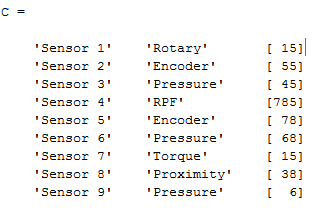
\includegraphics[width=.75\textwidth]{images/CUI}
	\caption{A sample of the CUI} 
	\label{fig:CUIV1}
\end{figure} 

\subsubsection{Graphical User Interface}

The (Graphical User Interface) was made using Matlab graphical elements. Initially, the GUI contained two tables, one which shows all the sensors and one which shows only a selection of important sensors. 
The table of important sensors is intended to show more details about the selected sensors while the table of all sensors is intended to give a quick overview of all sensors. The GUI contains two graphs as well which both plot the current as well as previous values of the selected sensor. When a sensor is selected in the table of all sensors, all properties of this sensor will be shown and can be edited. A property of special note is the 'SI-Prefix': in the table of important sensors, the SI-Prefix of a sensor can be changed, and the value will be scaled accordingly. 

\subsubsection{Limitations}

The Matlab UITable class has the disadvantage that the entire table has to be redrawn if something changes, even if only one cell changes. Since redrawing an entire table takes about $0.05$ seconds, 
doing this every update is not a possibility with an update rate of 50 Hz. Of course, having such an high update rate would make the table completely unreadable, since the data changes before one has even time to read it. In addition, in order to remove unnecessary redrawing, the static and dynamic parts of the tables are split where possible. Another problem introduced by the high refresh rate is that callback functions which are triggered by editing table cells do not function correctly. Because of the high update rate, the table is redrawn before the callback function has finished which gives unintended results. This problem has been solved by moving all cell with an edit callback to a table with a low refresh rate. 

\begin{figure}[H]
	\centering
	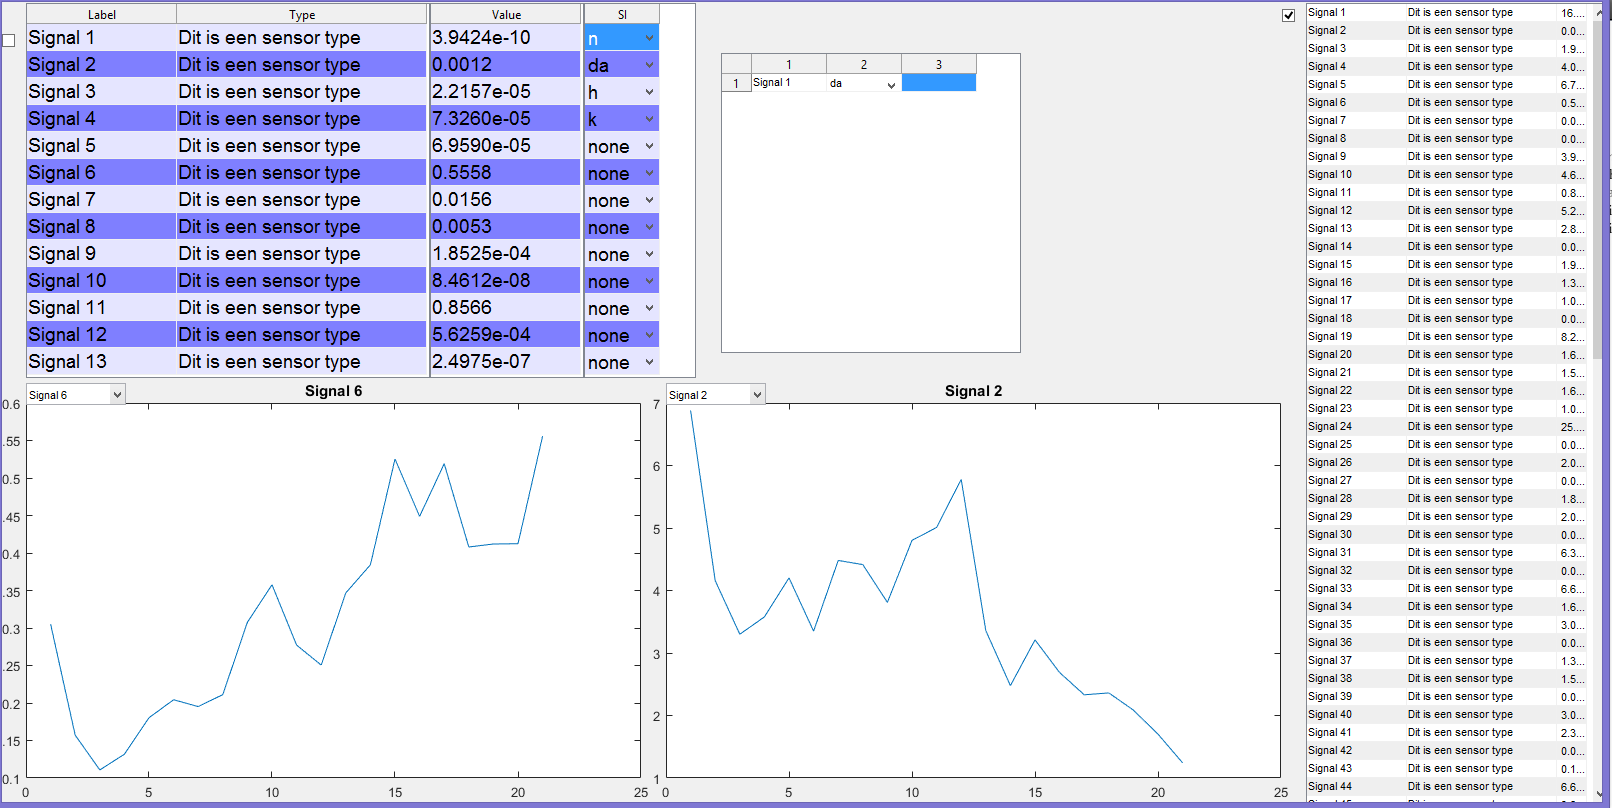
\includegraphics[width=.75\textwidth]{images/GUIV1}
	\caption{A sample of the GUI at the end of the second sprint} 
	\label{fig:GUIV1}
\end{figure} 

\subsection{Third Sprint}

\subsubsection{Visualisation}

For each sensor has an minimum and maximum safe value. When a value is not between these values, the sensor is marked red so it is immediately clear that there is something wrong. When a sensor is selected, one can see its minimum and maximum values. It is also possible to add multiple sensors to a graph in order to easily compare their values. It should be noted that the graphed data is not normalised, so visualising sensors with widely different data ranges is not advised.  

\subsubsection{Control}
The dimensions of all visual elements are static in order to have better control over the visual representation. To accommodate people with small screens, %we noemen geen namen
it is possible to toggle between two predefined sizes. These are defined in a separate configuration file which also contains other data which should be editable like the update rate of separate components and whether the sensor data is generated local or received over network. In the sensor property window, it is possible to toggle whether a sensor is in the table of important sensors. Additionally, a sensor can be given a transformation as well by entering the corresponding formula in the formula field in the sensor property window. 


\subsubsection{Limitations}
%TODO something something performance

\begin{figure}[H]
	\centering
	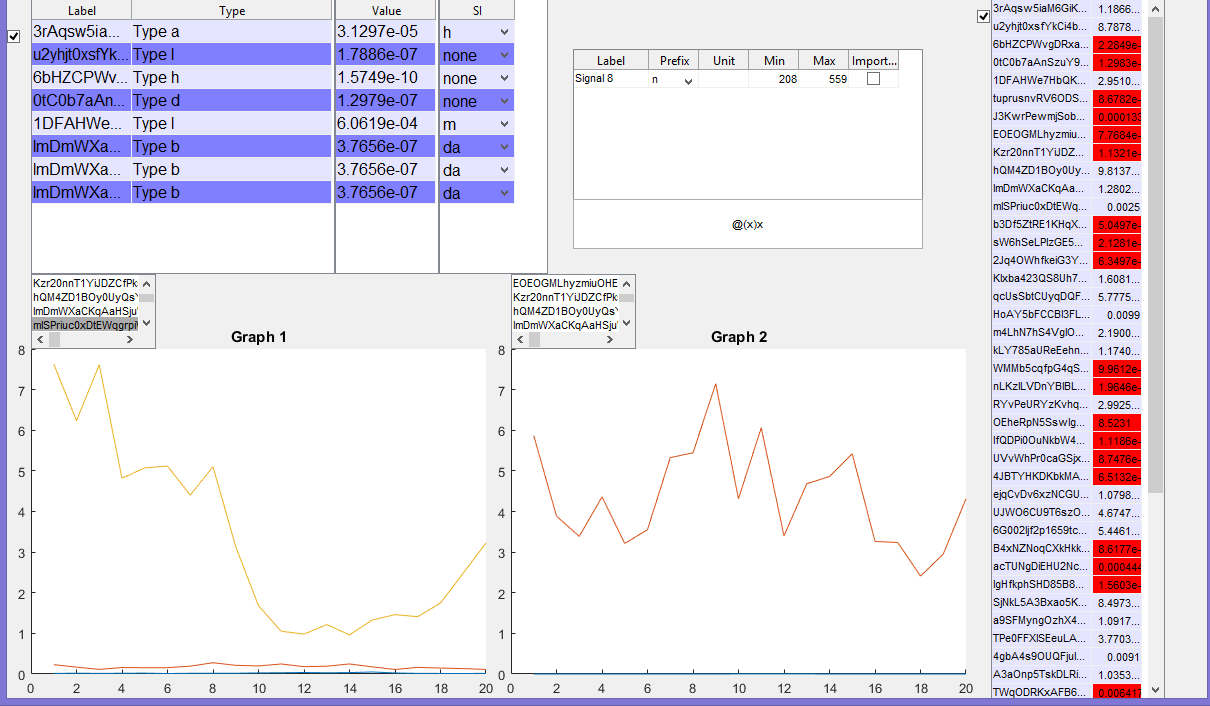
\includegraphics[width=.75\textwidth]{images/GUIV2}
	\caption{A sample of the GUI at the end of the third sprint} 
	\label{fig:GUIV2}
\end{figure} 

\subsection{Fourth Sprint}

\subsubsection{Performance}


